\documentclass[a4paper,11pt]{report}
\usepackage[margin=1.2in]{geometry}
\usepackage[latin1]{inputenc}
\usepackage[italian]{babel}
\usepackage{indentfirst}
\usepackage{mathtools}
\usepackage{amsmath}
\usepackage{amsfonts}
\usepackage{fancyhdr}
\usepackage{graphicx}
\usepackage{hyperref}
\newcommand{\virgolette}[1]{``#1''}
\newcommand{\N}{\mathbb{N}}
\newcommand{\Z}{\mathbb{Z}}
\newcommand{\addvar}[2]{% #1 name, #2 value
	\expandafter\def\csname varmacro#1\endcsname{#2}
}
\newcommand{\var}[1]{% 
	\csname varmacro#1\endcsname
}

\addvar{percorso_programma}{\url{http://formazione.comune.intranet}}

\addvar{nome_programma}{Formazione}

\addvar{mail_assistenza}{emidio.picariello@comune.fi.it}

\pagestyle{fancy}
\lhead{Manuale d'uso di \var{nome_programma}}
\lfoot{Emidio Picariello}
\rfoot{}

\title{Manuale d'uso di \var{nome_programma}}  
\author{Emidio Picariello \\ emidio.picariello@comune.fi.it }

\begin{document}
\maketitle

\newpage
\section*{Funzionalit�}
\subsection*{Accesso}

Il programma � attualmente testato per funzionare solo con Mozilla Firefox, scaricabile da qui \\
\begin{flushleft}
\url{http://www.mozilla.org/it/firefox/new/} \\ 
\end{flushleft}

Quando si accede collegandosi a \var{percorso_programma} il programma rinvia alla pagina di 
autenticazione di SSO (il sistema di Single Sign On del Comune). Qui si deve inserire la propria 
matricola e  la propria password. L'utente viene quindi automaticamente reindirizzato alla 
pagina successiva. 

\begin{flushleft}
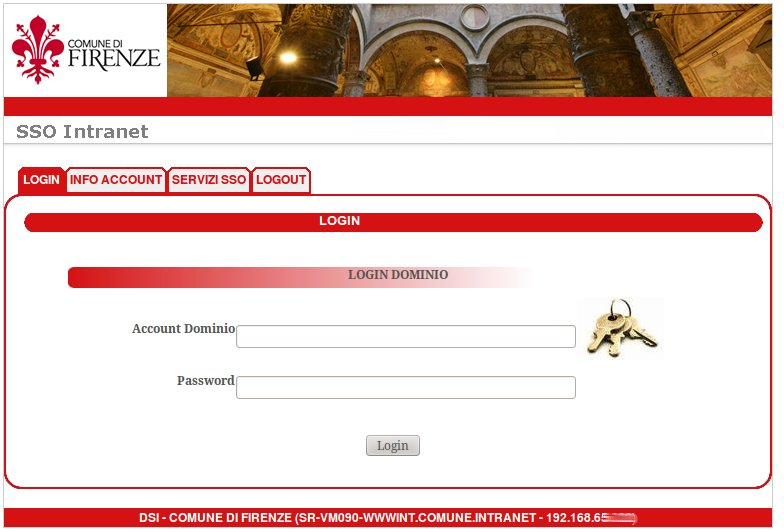
\includegraphics[scale=0.7]{img_gen/001_accesso.jpg}
\end{flushleft}
\newpage

\subsection*{Note generali}
Ciascuna pagina del programma � composta da un men� a tendina che mostra a ciascun utente 
solo le cose per le  quali esso dispone delle autorizzazioni e ogni voce di men� 
rimanda a una griglia che mostra i dati e offre le funzioni di ricerca e stampa. 

\begin{flushleft}
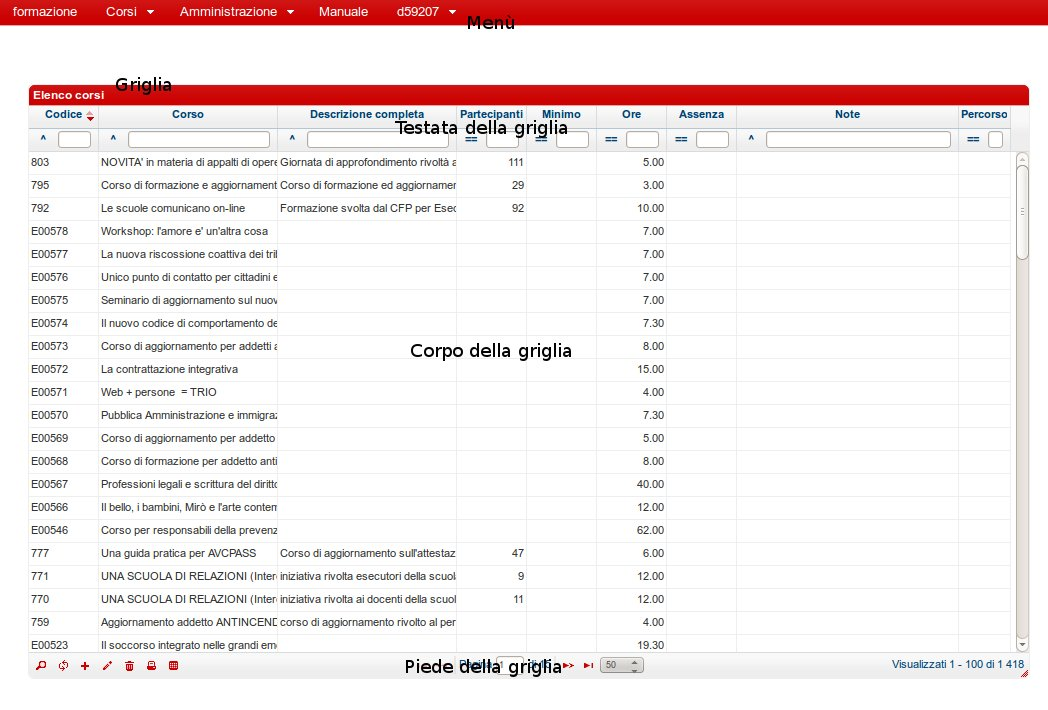
\includegraphics[scale=0.58]{img_gen/005_generale.jpg}
\end{flushleft}

Il men� � composto dal nome del programma (nell'esempio qui sotto \virgolette{Formazione}) 
come prima voce a sinistra, dalle voci di men� specifiche dell'applicazione e dalla voce
\virgolette{Manuale} (che consente di scaricare il presente manuale) e infine da una voce di men� 
caratterizzata dalla matricola che ha effettuato l'accesso. Cliccando sulla prima voce
(il nome del programma) si viene riportati alla pagina principale del programma, cliccando 
sul codice di matricola si apre un sotto-men� che consente di effettuare il \virgolette{Logout} (di uscire
dal programma in modo che altri utenti non lo possano utilizzare quando lasciamo incustodito 
il nostro computer). 

\begin{flushleft}

\includegraphics[scale=1]{img_gen/010_menu.jpg}
\end{flushleft}


Sopra ciascuna colonna (in quella che abbiamo chiamato \virgolette{Testata della griglia} 
� presente un campo di ricerca (nell'immagine qui sotto evidenziato in 
arancione) e un tasto che consente di selezionare il tipo di ricerca (qui sotto cerchiato in verde). 
Quando si clicca sul tasto \virgolette{tipo di ricerca} si apre un men� (qui sotto riquadrato di verde) dal 
quale possiamo scegliere che tipo di ricerca verr� effettuata. Per esempio: se seleziono il tipo 
di ricerca \virgolette{Inizia con} e nel campo di ricerca scrivo \virgolette{Pro}, la griglia mostrer� tutte le righe 
della mia tabella che, in quel campo hanno un valore che comincia con \virgolette{Pro} (\virgolette{Professionista}, 
\virgolette{Prototipo}, etc). Se invece scelgo \virgolette{Contiene} mostrer� tutte le righe che in quel campo contengono 
la parola \virgolette{pro} (\virgolette{Professionista}, \virgolette{Prototipo}, ma anche \virgolette{Apro}, etc.). 

Se clicco sul nome del campo (nell'esempio \virgolette{Corso}, riquadrato in giallo) verr� operato un ordinamento 
crescente (se clicco una volta), decrescente (se clicco una seconda volta), verr� annullato l'ordinamento
(se clicco una terza volta). Se effettuo queste operazioni su pi� campi i filtri si sommano e avr� una 
tabella filtrata secondo le mie esigenze. 

\begin{flushleft}
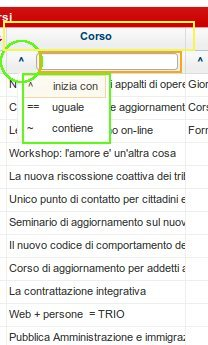
\includegraphics[scale=1]{img_gen/050_ricerca.jpg}
\end{flushleft}

Andiamo adesso a vedere come � composto il \virgolette{Piede della griglia}. A sinistra ci sono dei pulsanti 
che consentono di accedere ad alcune funzioni, nel  merito delle quali entreremo pi� avanti, al centro c'� 
il numero di pagina corrente e quante sono le righe mostrate in questa pagina. Qui si pu� anche scegliere di 
vedere pi� righe per ciascuna pagina. A destra c'� il conto delle righe mostrate rispetto alle righe totali 
della tabella (o rispondenti ai criteri di ricerca impostati). 

\begin{flushleft}
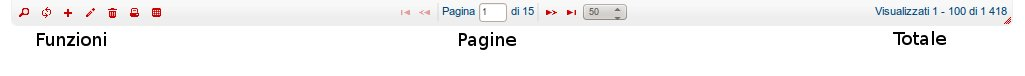
\includegraphics[scale=0.58]{img_gen/060_piede.jpg}
\end{flushleft}

Vediamo quindi le funzioni disponibili. Premettiamo che non tutte le funzioni sono disponibili in tutte 
le tabelle, quindi se una tasto non appare nella tabella in cui siete, semplicemente quella funzione 
non � disponibile per quella tabella. 

La prima funzione disponibile � quella di ricerca 
\includegraphics[scale=1]{img_gen/070_ricerca.jpg} che 
apre una pagina in cui si pu� compiere una ricerca ancora pi� avanzata di quella che si pu� 
effettuare dalla testata della griglia. Innanzitutto possiamo scegliere fra \virgolette{tutto} e 
\virgolette{almeno uno}. Poi possiamo aggiungere e togliere i campi sui quali vogliamo fare la 
ricerca con il simbolo \virgolette{+} accanto alla scelta fra \virgolette{tutto} e \virgolette{almeno uno} 
e con il simbolo \virgolette{-} accanto alla ricerca impostata. Possiamo inoltre scegliere il tipo di ricerca
(come nel caso della ricerca da testata della griglia si pu� cercare per inizio, contenuto, etc.) 

\begin{flushleft}
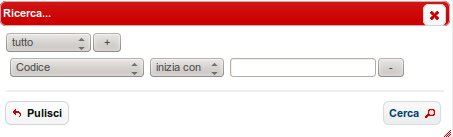
\includegraphics[scale=1]{img_gen/071_ricerca.jpg}
\end{flushleft}

Facciamo un esempio. Abbiamo una tabella con tre record. 

\begin{center}
\begin{tabular}{|c|c|} \hline
{$Nome$} & {$Cognome$}\\ \hline
Andrea & Manzi \\
Emidio & Picariello \\
Andrea & Rossi \\ \hline
\end{tabular} 
\end{center}

Se scelgo \virgolette{tutto} poi \virgolette{nome} \virgolette{inizia con} \virgolette{Andr} otterr� 

\begin{center}
\begin{tabular}{|c|c|} \hline
{$Nome$} & {$Cognome$}\\ \hline
Andrea & Manzi \\
Andrea & Rossi \\ \hline
\end{tabular}
\end{center}

Ovvero le due righe dove \virgolette{nome} inizia con \virgolette{Andr}

Se aggiungo \virgolette{cognome}, \virgolette{inizia con}, \virgolette{Ros}, ottengo solo \virgolette{Andrea Rossi} 
ovvero la riga che soddisfa tutti i criteri (ricordiamo che ho scelto \virgolette{tutto}). 

Se invece scelgo \virgolette{almeno uno} e poi scelgo \virgolette{cognome} \virgolette{inizia con} \virgolette{man} 
poi clicco su \virgolette{+} e aggiungo una riga \virgolette{cognome} \virgolette{inizia con} \virgolette{pica} ottengo

\begin{center}
\begin{tabular}{|c|c|} \hline
{$Nome$} & {$Cognome$}\\ \hline
Andrea & Manzi \\
Emidio & Picariello \\ \hline
\end{tabular}
\end{center}

ovvero tutte le righe che soddisfano almeno uno dei due criteri che ho impostato. 

Cliccando sul tasto 	\virgolette{pulisci} ottengo la cancellazione di della ricerca. Notiamo che effettuo una ricerca
e poi chiudo la finestra di ricerca, la ricerca resta impostata sulla pagina e in basso, appare la scritta: 

\begin{flushleft}
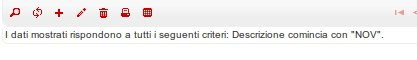
\includegraphics[scale=1]{img_gen/072_ricerca.jpg}
\end{flushleft}

In questo modo siamo consapevoli del fatto che non stiamo vedendo tutti i dati e che per vedere tutti i dati dobbiamo 
cliccare di nuovo su 
\includegraphics[scale=1]{img_gen/070_ricerca.jpg} e poi su \virgolette{Pulisci}

La seconda funziona che troviamo � rappresentata dal simbolo 
\includegraphics[scale=1]{img_gen/075_refresh.jpg} che ha lo 
scopo di ricaricare i dati della griglia. Questo potrebbe essere necessario se qualcun altro da un'altra postazione 
aggiunge o modifica i dati. 

La funzione successiva, rappresentata dal simbolo 
\includegraphics[scale=1]{img_gen/080_piu.jpg} consente di aggiungere 
una riga. Ci� pu� avvenire o tramite una apposita maschera, o con la possibilit� di immissione dei dati direttamente 
all'interno di una riga bianca della griglia che in questo caso apparir�. In quel caso avremo altre due icone di funzione
ovvero quella per salvare 
\includegraphics[scale=1]{img_gen/086_salva.jpg} la modifica effettuata sulla riga e 
quella per annullare la modifica 
\includegraphics[scale=1]{img_gen/087_annulla.jpg}.

Ma di questo si parler� pi� dettagliatamente quando parleremo di ciascuna funzionalit�. 

Successivamente troviamo la funzione 
\includegraphics[scale=1]{img_gen/081_edit.jpg} di modifica che consente di modificare 
una riga esistente dopo averci cliccato una volta. Si accede alla funzione di modifica anche cliccando due volte su una 
riga. La funzione rappresentata dal tasto 
\includegraphics[scale=1]{img_gen/082_delete.jpg} � quella classica di cancellazione. 

Le operazioni di aggiunta, modifica e cancellazione si posso attivare anche cliccando con il tasto destro su una riga, si 
apre quindi un men�: 

\begin{flushleft}
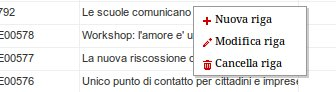
\includegraphics[scale=1]{img_gen/090_tasto_destro.jpg}
\end{flushleft}

Cliccando sul pulsante 
\includegraphics[scale=1]{img_gen/083_stampa.jpg} si ottiene la stampa delle informazioni che si trovano 
nella griglia in quel momento, in formato pdf. La funzione 
\includegraphics[scale=1]{img_gen/084_custom.jpg} invece apre una 
maschera che mostra tutti i campi della tabella e permette di scegliere quali mostrare in griglia. 

\begin{flushleft}
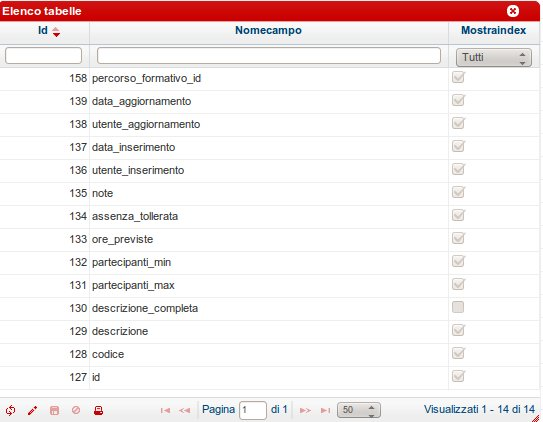
\includegraphics[scale=1]{img_gen/085_custom.jpg}
\end{flushleft}

Dopo aver selezionano la riga che si desidera modificare si clicca su 
\includegraphics[scale=1]{img_gen/081_edit.jpg} si 
toglie o si aggiunge la spunta alla colonna che si vuole nascondere o mostrare e poi si 
salva 
\includegraphics[scale=1]{img_gen/086_salva.jpg} \footnote{Alcuni campi non possono essere mostrati in griglia 
a causa di una impostazione specifica del programma. In quel caso, anche se appare la spunta in questa finestra
comunque non appariranno. In questo caso si pu� concordare con gli sviluppatori del software una modifica di 
questa impostazione, ma non � una modifica che l'utente pu� apportare autonomamente.}. Le impostazioni cos� effettuate 
avranno valore solo per l'utente che le ha effettuate e non per tutti gli utenti.  




\newpage
\section*{Segnalazione degli Errori}
\subsection*{Il software Mantis}
Per segnalare gli errori o le richieste di intervento in modo che vengano visualizzati e gestiti dagli sviluppatori 
� necessario accedere alla pagina: 

\url{http://mantis.comune.intranet/}

Dalla quale si viene come al solito rimandati alla pagina di autenticazione.

\begin{flushleft}
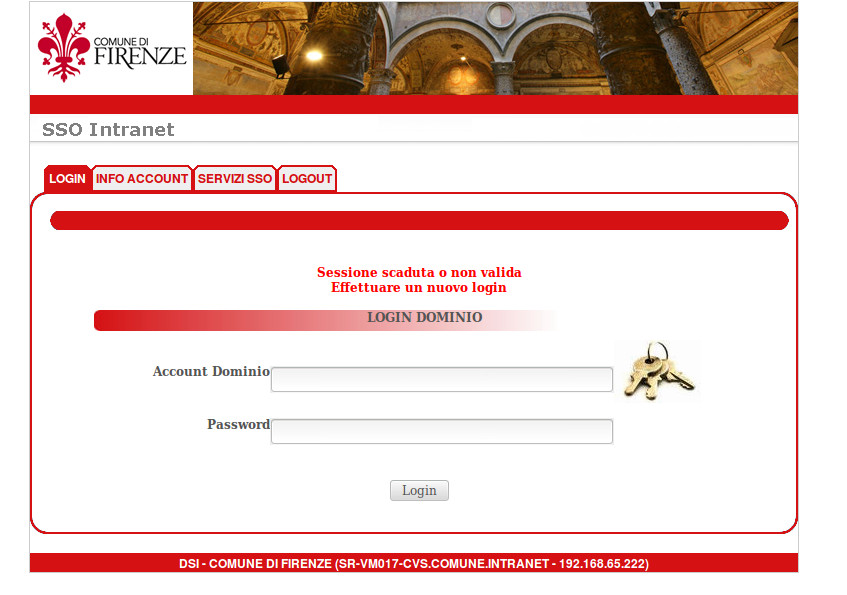
\includegraphics[scale=0.7]{img_mantis/001_sso.jpg}
\end{flushleft}

Se si era gi� autenticati o se il ci si � autenticati il programma rimanda alla pagina iniziale di Mantis. 

\begin{flushleft}
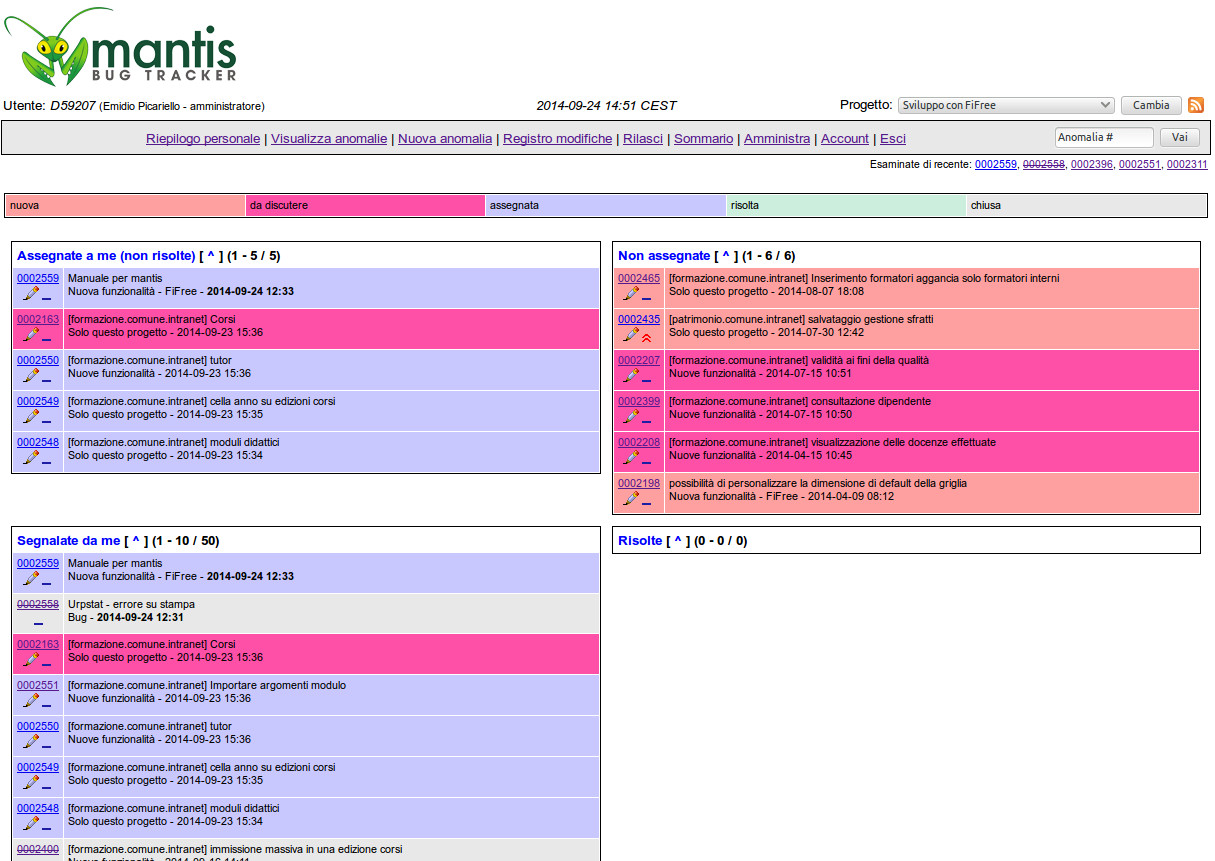
\includegraphics[scale=0.5]{img_mantis/010_home.jpg}
\end{flushleft}

Se non si � indirizzati a questa pagina, scrivere una mail a \var{mail_assistenza} indicando il proprio numero di matricola, il proprio nome
la propria email completa e il programma per il quale si vuole essere abilitati alla segnalazione di errori o migliorie. \\

La pagina che ci si trova di fronte ha in alto a destra il nome del progetto (se siete abilitati a pi� progetti scegliete l� per quale progetto 
state facendo la segnalazione). 

\begin{flushleft}
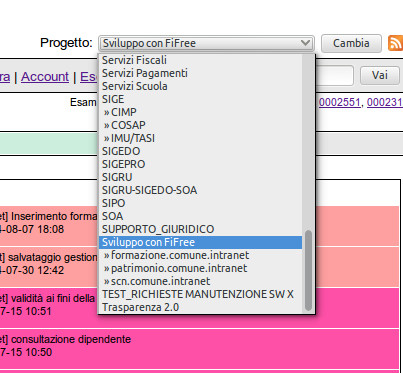
\includegraphics[scale=0.7]{img_mantis/020_progetto.jpg}
\end{flushleft}

Nel corpo della pagina vedrete le segnalazioni che avete fatto e il loro stato, indicato dal colore: 

\begin{flushleft}
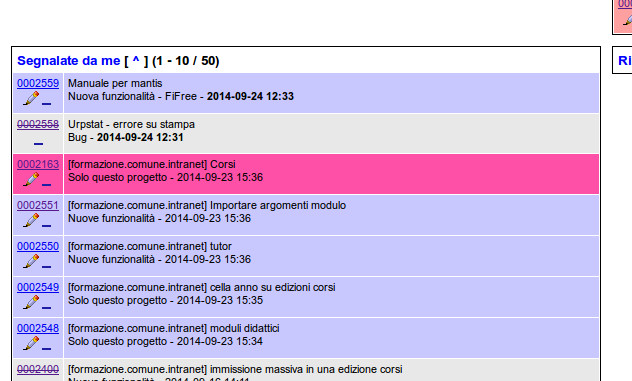
\includegraphics[scale=0.7]{img_mantis/030_segnalate.jpg}
\end{flushleft}

Nel men� avete invece la possibilit� di cliccare su \virgolette{Nuova Anomalia} che apre la pagina nella quale potete immettere la nuova 
richiesta: 

\begin{flushleft}
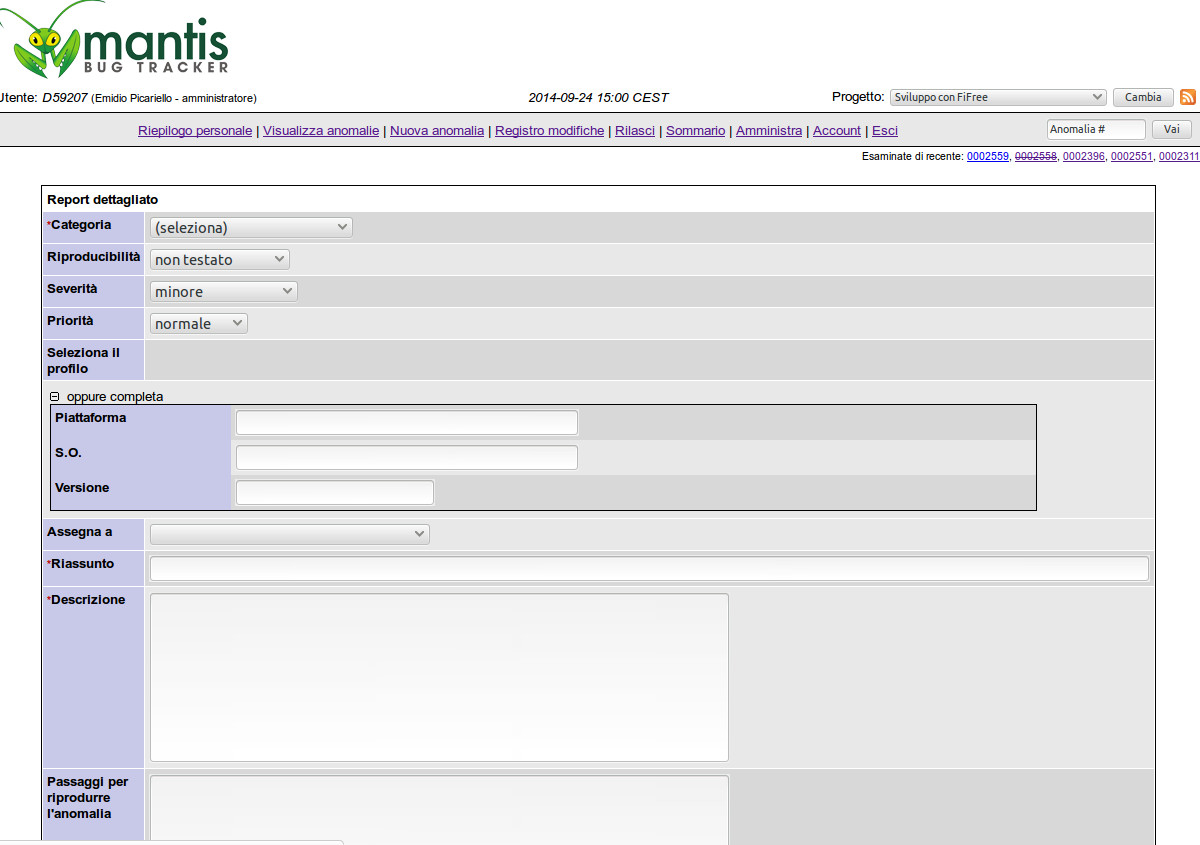
\includegraphics[scale=0.5]{img_mantis/050_segnala.jpg}
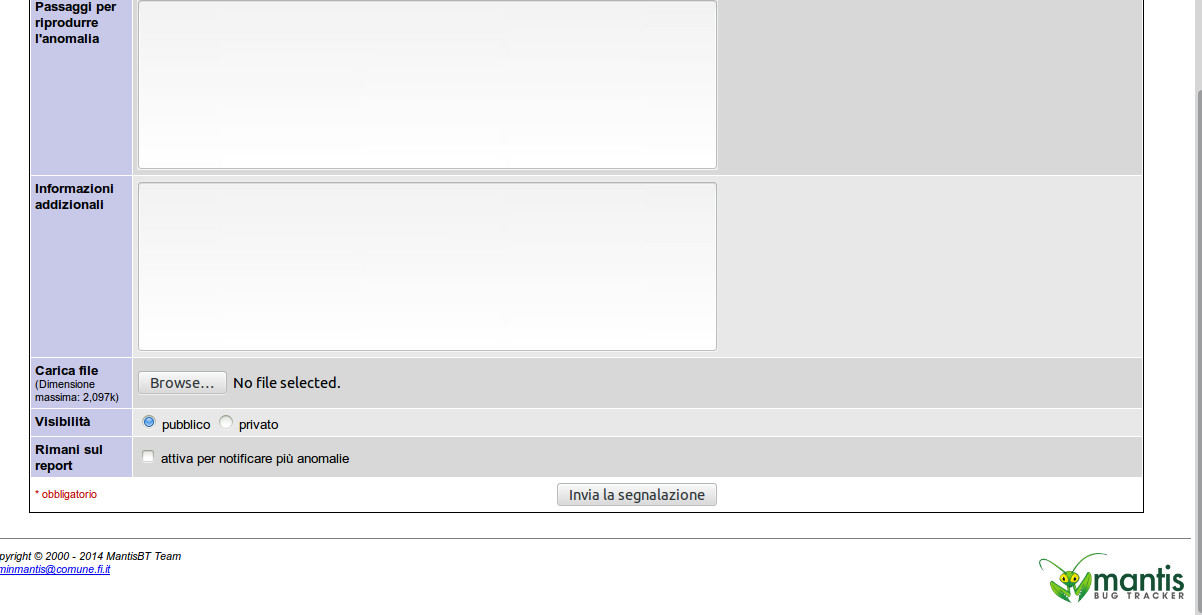
\includegraphics[scale=0.5]{img_mantis/055_segnala.jpg}
\end{flushleft}

I campi contrassegnati dall'asterisco sono obbligatori. Per fare una buona segnalazione � necessario ragionare attentamente sulle 
informazioni che si forniscono e su quelle che si omettono. Nel campo \virgolette{categoria}si sceglie la categoria pi� appropriata 
fra quelle che sono disponibili per il progetto. Nel campo \virgolette{riproducibilit�} si 
segnala se l'errore si verifica tutte le volte che si fa una determinata operazione o se si verifica solo ogni tanto 
o se si � verificato una volta ma non si � in grado di riprodurlo. I due campi successivi sono diversi e molto importanti: 
la \virgolette{severit�} di un errore ha a che fare con quanto grave �. Le voci sono in ordine di gravit�, \virgolette{crash} significa
che il programma si chiude quando si verifica quell'errore, \virgolette{blocco} significa che non c'� modo di andare avanti. 
Il campo \virgolette{priorit�} invece indica quanto urgente � l'errore o la richiesta. Chiaramente ci deve essere un grado. 
Se tutte le richieste sono segnalate come \virgolette{immediata} o \virgolette{urgente} chi deve farsene carico non sapr� da quale cominciare. 
Per esempio: se lancio una stampa una volta l'anno e i dati di quella stampa sono sbagliati, l'errore sar� di gravit� \virgolette{maggiore} 
ma la priorit� sar� \virgolette{normale}. \\
I dati relativi a piattaforma e sistema operativo si possono normalmente omettere a meno che non si debba comunicare qualcosa che il programmatore non 
sa (i programmi si usano con Firefox su Windows, se ho un Mac e uso Safari, lo devo scrivere qui). \\
Il riassunto deve essere breve e indicare che cosa accade, invece nella descrizione � importante scrivere dove ci si trova (per esempio) 
\virgolette{Tabelle} $\rightarrow$ \virgolette{Anagrafiche}. Se si scrive per esempio \virgolette{non controlla la data} questo sar� un errore impossibile da correggere. 
Che vuol dire? Cosa dovrebbe controllare? In che pagina si verifica l'errore? Invece \virgolette{in anagrafica cliente non controlla che la 
data di nascita sia anteriore a 18 anni fa per verificare che il soggetto immesso abbia la maggiore et�} � un errore segnalato correttamente. 
Pi� i dati sono corretti e completi e pi� veloce sar� la risoluzione del problema. \\
Una volta immessi tutti i dati basta cliccare su \virgolette{Invia la segnalazione} 

\newpage

\begin{flushleft}
Per la stesura di questa relazione sono stati utilizzati i seguenti strumenti opensource: \\

\LaTeX\ \url{http://www.latex-project.org/} \\
Texmaker \url{http://www.xm1math.net/texmaker/} \\
Gimp \url{http://www.gimp.org/} \\

\end{flushleft}

\end{document}